\documentclass[11pt]{article}

\usepackage[a4paper,margin=0.9in]{geometry}
\usepackage{amsmath,amssymb}
\usepackage{booktabs,tabularx,array}
\usepackage{enumitem}
\usepackage{tikz}
\usepackage{xcolor}
\usepackage{microtype}
\usepackage{hyperref}
\usetikzlibrary{arrows.meta,positioning}

\hypersetup{colorlinks=true,linkcolor=blue,urlcolor=blue,citecolor=blue}
\setlength{\parindent}{0pt}
\setlength{\parskip}{4pt}
\setlist{nosep,leftmargin=*}
\renewcommand{\arraystretch}{1.12}

\title{Missing-Value Imputation with GAIN\\\large Implementation, Evaluation, and Baseline Comparison}
\author{[Student Name]\\[Course / Group]}
\date{\today}

\begin{document}
\maketitle

\begin{abstract}
This project implements a tabular missing-value imputation workflow based on Generative Adversarial Imputation Nets (GAIN) and compares it with mean and median baselines. The workflow pairs incomplete records with complete reference data, preserves a mask of missing positions, applies a shared preprocessing schema, imputes values, and evaluates numeric and categorical attributes using the metrics specified in the project instructions. Numeric values are assessed with normalized root mean square error (NRMS); categorical values are assessed with exact-match accuracy (AE). Corrected-code results are reported for ten numeric Iris variants and one representative categorical, mixed, and numeric case. On the ten Iris variants, the simple baselines achieve lower mean NRMS than GAIN. The limited results therefore do not support a claim that GAIN is generally superior; broader repeated experiments are needed.
\end{abstract}

\section{Introduction}
Incomplete tabular data can limit downstream analysis and modeling. This project studies whether a neural imputation method can recover deliberately removed values and how it compares with simple column-wise statistics. The objectives are to implement GAIN, preserve the locations of missing values during preprocessing and output, support both numeric and categorical attributes, and compare the learned method with mean and median imputation.

The repository contains 26 complete source workbooks and corresponding incomplete dataset variations. This report does not claim that all available variations have been rerun with the corrected metrics. Its quantitative evidence consists of the ten Iris variants in the current comparison workbook and verified single-run examples for HOV, Abalone, and 4-gauss. This scope distinction is important when interpreting the results.

\section{Related Work}
Generative Adversarial Imputation Nets (GAIN), introduced by Yoon, Jordon, and van der Schaar, adapt generative adversarial learning to incomplete tabular data. GAIN trains a generator to propose values at missing positions and a discriminator to distinguish observed from imputed entries. A hint mechanism reveals partial mask information to the discriminator, encouraging it to learn feature-level observation patterns \cite{yoon2018gain}.

The adversarial approach is motivated by the fact that missingness patterns and relationships among columns can carry information about plausible values. Rather than minimizing a reconstruction loss on unknown entries, which have no observed target during training, GAIN uses the discriminator's ability to distinguish observed from generated entries as an indirect learning signal. Its hint mechanism limits the discriminator's certainty about the mask so it must learn from the joint data distribution.

This project compares that learned approach with two univariate statistical baselines: replacing a missing numeric value with its feature mean or median, and replacing a missing categorical value with its feature mode. Such statistics are commonly used as simple reference methods because they are transparent and computationally inexpensive. They do not model relationships among features, but can perform well when attributes are weakly related, the dataset is small, or a numeric column is concentrated around its center. Including them helps distinguish the value of the learned model from the value of merely filling every gap.

The evaluation follows the course handout rather than treating AE as an absolute-error quantity: in this project, AE denotes categorical exact-match accuracy, while NRMS measures numeric imputation error. This distinction also motivates recording execution time in a separate field. The study is an implementation and comparison exercise; it does not introduce a new imputation algorithm.

\section{Methodology}
\subsection{Dataset and Preprocessing}
Input spreadsheets are read without a header row so that the matrix coordinates remain unchanged. For each experiment, the incomplete table is paired with its complete reference table. The program checks that the two tables have matching shapes and creates a mask $M$ with $M_{ij}=1$ for an observed value and $M_{ij}=0$ for a missing value.

Categorical values are mapped to integer codes using the complete reference data so that the incomplete and reference tables share the same encoding. A Min-Max scaler is fitted on the complete matrix and then applied to the incomplete matrix. Missing entries in the scaled model input are set to zero; their original missing locations remain available in the mask. After imputation, numeric values are inverse-transformed and categorical codes are rounded to a valid code and restored to their original labels. Only missing cells are written into the output table.

The current type rule treats string-like columns as categorical and integer-valued columns with at most 20 distinct values as categorical. The \texttt{Letter} pixel features are explicitly marked numeric. The per-dataset \texttt{FEATURE\_TYPE\_OVERRIDES} setting supports corrections when a numeric-coded category or a low-cardinality numeric measurement would otherwise be misclassified. This heuristic requires review for datasets whose column semantics are not clear from their values alone.

\begin{table}[ht]
\centering
\small
\caption{Representative source datasets used in the corrected-code checks.}
\begin{tabularx}{\linewidth}{l l c X}
\toprule
Dataset & Feature composition & Shape & Evaluation role \\
\midrule
Iris & Numeric & $150\times4$ & Ten missing-data variants; aggregate comparison \\
HOV & Categorical & $232\times16$ & Categorical accuracy example \\
Abalone & Mixed & $4177\times8$ & Numeric and categorical metric example \\
4-gauss & Numeric & $800\times12$ & Numeric NRMS example \\
\bottomrule
\end{tabularx}
\end{table}

\subsection{Methodology Steps and Workflow}
Each experiment follows the same sequence so that GAIN and the baselines see the same incomplete input and are scored against the same reference:
\begin{enumerate}
  \item Pair one incomplete workbook with its complete original workbook and verify that their row and column dimensions agree.
  \item Create a binary mask before any filling. The mask records the exact missing coordinates and is carried through preprocessing and evaluation.
  \item Infer or configure column types, encode categorical labels using the complete reference, and fit the Min-Max scaler on that reference. Transform the incomplete matrix using the same schema; use zero only as a model-input placeholder for missing values.
  \item Run GAIN, Mean, and Median on the same matrix and mask. For categorical columns, the statistical baselines use the mode rather than arithmetic on category codes.
  \item Restore numeric values and category labels, insert predictions only at masked positions, calculate the applicable metrics, and save imputed workbooks and Excel score tables.
\end{enumerate}

This sequence was developed to avoid two practical sources of invalid results: shifting imputed values away from their original spreadsheet coordinates, and comparing categories encoded differently in the incomplete and reference files. Fitting the encoding and scaler on the complete reference makes their transformations consistent. The mask is never reconstructed from the filled model input; it remains the source of truth for which cells are to be scored and replaced.

Batch evaluation updates the results workbook, while comparison mode runs GAIN, Mean, and Median and saves Excel score tables and imputed datasets. Progress and runtime estimates are printed for long runs. Figure~\ref{fig:workflow} summarizes the processing sequence.

\begin{figure}[ht]
\centering
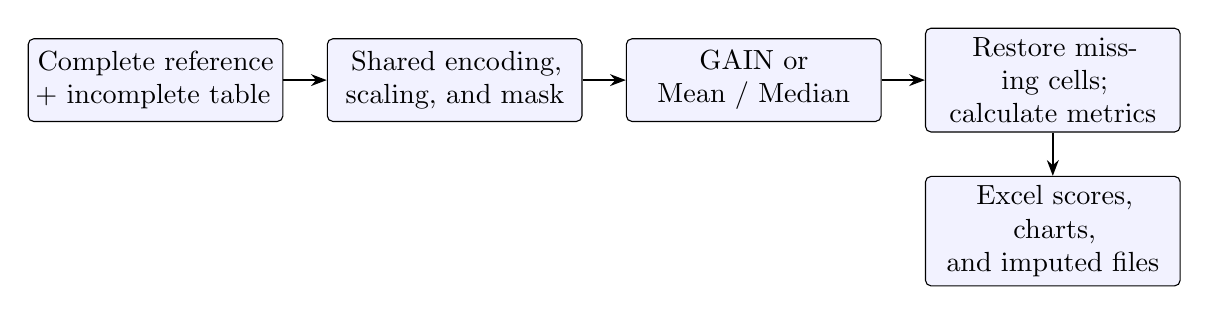
\begin{tikzpicture}[
  block/.style={draw,rounded corners=2pt,align=center,text width=3.0cm,minimum height=1.05cm,fill=blue!5},
  arrow/.style={-{Stealth[length=2mm]},thick},
  node distance=0.55cm and 0.55cm
]
\node[block] (input) {Complete reference\\+ incomplete table};
\node[block,right=of input] (prepare) {Shared encoding,\\scaling, and mask};
\node[block,right=of prepare] (impute) {GAIN or\\Mean / Median};
\node[block,right=of impute] (evaluate) {Restore missing cells;\\calculate metrics};
\draw[arrow] (input) -- (prepare);
\draw[arrow] (prepare) -- (impute);
\draw[arrow] (impute) -- (evaluate);
\node[block,below=of evaluate,text width=3.0cm] (output) {Excel scores, charts,\\and imputed files};
\draw[arrow] (evaluate) -- (output);
\end{tikzpicture}
\caption{End-to-end imputation and evaluation workflow.}
\label{fig:workflow}
\end{figure}

For reproducibility, comparison runs can be launched from the project directory with:
\begin{verbatim}
source venv/bin/activate
python3 main.py --compare --dataset Iris_C_1
python3 main.py --compare --dataset Abalone_C_1
python3 main.py --compare --dataset HOV_NL_1
\end{verbatim}
The default comparison workbook is \texttt{comparison\_results.xlsx}.

\subsection{GAIN and Mean and Median}
The implementation uses a generator and discriminator. The generator receives the partially observed matrix $\bar{X}$, mask $M$, and random noise $Z$. Its multilayer perceptron has two ReLU hidden layers of width $2d$ for an input with $d$ features, followed by a sigmoid output. Observed entries are copied through unchanged:
\[
\hat{X}=M\odot\bar{X}+(1-M)\odot G(\bar{X},M,Z).
\]
A hint matrix $H$ provides partial information about the mask to the discriminator, which receives the completed sample and hint and predicts whether values were observed. This adversarial interaction encourages the generator to produce plausible missing values.

Training alternates discriminator and generator updates over shuffled mini-batches. For the discriminator update, the generator creates a completion and the discriminator is trained against the observed/missing mask, with the hint matrix providing partial mask information. For the generator update, the discriminator's response on missing cells contributes an adversarial objective. A reconstruction term on observed cells helps retain the input values during training. At inference, the trained generator is applied with a newly sampled noise matrix, and its mask-weighted output retains observations while supplying estimates in the missing cells.

The discriminator objective is a mask-prediction binary cross-entropy. The generator combines an adversarial term on missing entries with a reconstruction term on observed entries:
\begin{align*}
L_D &= -\mathbb{E}\left[M\log D(\tilde{X},H)+(1-M)\log(1-D(\tilde{X},H))\right],\\
L_G &= -\mathbb{E}\left[(1-M)\log D(\tilde{X},H)\right]
       +\alpha\frac{\sum M\odot(X-\hat{X})^2}{\sum M}.
\end{align*}
The current comparison configuration uses 200 epochs, batch size 32, hint probability 0.9, $\alpha=100$, and Adam with learning rate $0.001$. Model initialization and random noise are not fixed to a seed, so repeated runs can vary.

\paragraph{Mean and Median baselines.}
Mean and median baselines are computed feature by feature from observed values under the same mask as GAIN. Numeric features receive their observed mean or median. Categorical features receive the observed mode; averaging category codes would not yield a meaningful category. All methods are scored against the same complete reference data.

\subsection{Evaluation Metrics}
For numeric features, the instructions define NRMS as the normalized Frobenius error. Let $\Omega_N$ be the set of missing numeric cells, and let $X_N$ contain the complete numeric reference values. The code computes the error only at missing cells and normalizes it by the norm of the complete numeric reference matrix:
\[
\mathrm{NRMS}=\frac{\left(\sum_{(i,j)\in\Omega_N}(x_{ij}-\hat{x}_{ij})^2\right)^{1/2}}{\|X_N\|_F}.
\]
This is equivalent to the full numeric-matrix difference in the instruction because observed values are copied through unchanged. Lower NRMS is better.

For categorical features, AE is exact-match accuracy over missing categorical cells $\Omega_C$:
\[
\mathrm{AE}=\frac{1}{|\Omega_C|}\sum_{(i,j)\in\Omega_C}\mathbf{1}[x_{ij}=\hat{x}_{ij}].
\]
AE lies between zero and one; higher is better. A metric is left blank when no missing cells of its feature type are present. Imputation runtime is stored separately as \texttt{Runtime\_s}; it is not AE.

\section{Results and Discussion}
\subsection{Ten Numeric Iris Variants}
The current root comparison workbook contains ten Iris variants with missing rates from approximately 0.67\% to 20\%. Table~\ref{tab:iris} reports the mean NRMS and mean computation time across those variants. Mean achieves the lowest average NRMS, followed closely by Median; GAIN has the highest average NRMS. The best NRMS is achieved by Mean on six variants and Median on four; GAIN is not best on any of these ten cases. Table~\ref{tab:iris-detail} lists every observed variant score so that the aggregate can be inspected against individual cases.

\begin{table}[ht]
\centering
\small
\caption{Average results over ten numeric Iris variants. Runtime is the measured imputation computation time, not total file-processing time.}
\label{tab:iris}
\begin{tabular}{lrrr}
\toprule
Method & Mean NRMS $\downarrow$ & Mean runtime & Best NRMS cases \\
\midrule
GAIN   & 0.0928 & 0.582 s  & 0/10 \\
Mean   & 0.0581 & 0.031 ms & 6/10 \\
Median & 0.0586 & 0.128 ms & 4/10 \\
\bottomrule
\end{tabular}
\end{table}

The GAIN mean NRMS is about 60\% higher than the Mean baseline in this subset. The baselines are expected to be much faster because their imputation step is a simple column statistic, whereas GAIN trains a neural network for each dataset. The result indicates that model complexity alone did not improve accuracy on these Iris cases.

\begin{table}[ht]
\centering
\small
\caption{NRMS for each verified Iris variant. Lower values indicate better numeric imputation.}
\label{tab:iris-detail}
\begin{tabular}{lrrrr}
\toprule
Variant & Missing rate & GAIN & Mean & Median \\
\midrule
Iris\_AE\_1  & 0.67\% & 0.0249 & 0.0234 & 0.0223 \\
Iris\_AE\_5  & 4.67\% & 0.0755 & 0.0465 & 0.0463 \\
Iris\_AE\_10 & 9.33\% & 0.1112 & 0.0715 & 0.0713 \\
Iris\_AE\_20 & 19.00\% & 0.1551 & 0.0971 & 0.0980 \\
Iris\_AG\_1  & 0.67\% & 0.0350 & 0.0163 & 0.0170 \\
Iris\_AG\_5  & 4.67\% & 0.0501 & 0.0450 & 0.0470 \\
Iris\_C\_1   & 1.00\% & 0.0636 & 0.0321 & 0.0327 \\
Iris\_C\_5   & 5.00\% & 0.1390 & 0.0699 & 0.0678 \\
Iris\_C\_10  & 10.00\% & 0.1316 & 0.0741 & 0.0783 \\
Iris\_C\_20  & 20.00\% & 0.1422 & 0.1050 & 0.1050 \\
\bottomrule
\end{tabular}
\end{table}

Across these ten variants, the Mean baseline lowers average NRMS by about 37\% relative to GAIN; equivalently, GAIN's mean NRMS is about 60\% higher than Mean's. The average difference between Mean and Median is small (approximately 0.0005 NRMS), indicating that their aggregate performance is nearly tied even though their per-variant wins differ. The standard deviations across variants are 0.0486 for GAIN, 0.0302 for Mean, and 0.0305 for Median. GAIN therefore has both a higher average error and a wider spread across this subset. These standard deviations describe differences among the ten variants, not uncertainty from repeated training on the same variant.

NRMS generally rises as more cells are removed within the AE series, but the pattern is not strictly monotonic for every method or missingness mechanism. The C and AG series also differ from AE in which cells are removed, so missing rate alone cannot explain their scores. A fair interpretation should consider the exact mask pattern as well as the percentage missing.

\subsection{Categorical, Mixed, and Numeric Examples}
Table~\ref{tab:types} gives three additional corrected-code runs. HOV has categorical attributes only, 4-gauss has numeric attributes only, and the Abalone variation contains both. The results show that both metrics are produced for a mixed case, while the inapplicable metric remains blank for single-type cases.

\begin{table}[ht]
\centering
\small
\caption{One verified run per method for representative feature types. NRMS is lower-is-better; AE is higher-is-better.}
\label{tab:types}
\begin{tabular}{llrrr}
\toprule
Dataset & Method & NRMS & AE & Runtime (s) \\
\midrule
HOV\_NL\_1 & GAIN   & --     & 0.4500 & 2.0304 \\
           & Mean   & --     & 0.5000 & 0.0006 \\
           & Median & --     & 0.5000 & 0.0002 \\
\midrule
Abalone\_C\_1 & GAIN   & 0.1306 & 0.1765 & 18.6102 \\
              & Mean   & 0.0439 & 0.5000 & 0.0006 \\
              & Median & 0.0436 & 0.5000 & 0.0016 \\
\midrule
4-gauss\_AL\_5 & GAIN   & 0.4008 & --     & 4.1811 \\
               & Mean   & 0.1785 & --     & 0.0001 \\
               & Median & 0.1871 & --     & 0.0003 \\
\bottomrule
\end{tabular}
\end{table}

In the mixed Abalone case, both baselines outperform GAIN on numeric NRMS and categorical AE. The AE values of 0.50 for Mean and Median mean that half of the missing categorical entries were filled exactly in this run; the GAIN value of 0.1765 indicates substantially fewer exact matches. In the numeric 4-gauss case, both baselines also achieve lower NRMS. On HOV, the two mode baselines reach 0.50 categorical accuracy versus 0.45 for GAIN. These are individual runs, not averages over repeated random seeds. In particular, a mode baseline can attain a high categorical accuracy when one class is common, so class balance and per-feature results should be examined in a larger study.

The ten Iris variants favor Mean or Median, and the selected categorical and mixed examples also favor the mode-based baselines on AE. The numeric 4-gauss example favors both baselines on NRMS. These results suggest that simple per-feature statistics are strong on the tested cases, while GAIN's greater computational cost did not translate into better imputation accuracy in this limited sample. This is not evidence that GAIN is generally inferior; the analysis is restricted to the listed datasets and configurations.

In computational terms, for $N$ rows, $d$ features, and $E$ epochs, the dense GAIN network has approximately $O(ENd^2)$ training work, in addition to discriminator and generator passes. The column-wise baselines require approximately $O(Nd)$ work. Both methods store at least the data and mask, requiring $O(Nd)$ memory, while GAIN also stores network parameters and batch activations. The measured runtimes in the tables are illustrative local timings; preprocessing, Excel writing, and chart generation are excluded from the per-method timer.

\section{Limitations}
Only ten Iris variants and one selected case for each of HOV, Abalone, and 4-gauss were used here; the remaining dataset variations require a corrected full batch run. GAIN training is stochastic and each reported case is a single run, so results should be repeated across seeds and summarized with variability. Feature types are partly inferred from data values; explicit overrides should be checked against dataset documentation. Finally, ordinal encoding and rounding for nominal categories imposes an artificial order on category labels. One-hot or categorical-specific output layers would be a more principled extension.

\section{Conclusion}
This project delivers a mask-aware GAIN imputation pipeline, Mean and Median baselines, type-specific evaluation, and Excel-ready outputs. The metric implementation now follows the assignment convention: numeric missing values are scored with NRMS, categorical missing values with exact-match AE, and model runtime is reported separately. In the corrected results examined for this report, the simple baselines outperform GAIN on average for the Iris variants and on the selected numeric and mixed examples. The next steps are to verify feature typing for all datasets, run the complete corrected experiment set, repeat stochastic GAIN runs with fixed and varied seeds, and then update the result analysis before submission.

\begin{thebibliography}{9}
\bibitem{yoon2018gain}
J. Yoon, J. Jordon, and M. van der Schaar,
\newblock ``GAIN: Missing Data Imputation using Generative Adversarial Nets,''
\newblock in \emph{Proceedings of the 35th International Conference on Machine Learning}, PMLR, vol. 80, pp. 5689--5698, 2018.

\bibitem{assignment}
\newblock \emph{Instructions}, project assignment handout, provided with the course project.
\end{thebibliography}

\end{document}
